\cite{ARCADIA-Pancheri}
\cite{ARCADIA-Pancheri2}

Breve introduzione analoga a Monopix1 in cui descrivo brevemente la "timeline" da SEED Matisse a Md1 e Md2

Tutti i minid, siano essi v1 o v2, sono Alpide like.
Prima SEED si occupa di studiare le prestazioni: oncept study with small-scale test structure (SEED),
dopo arcadia: technology demonstration with large area sensors
Small scale demo SEED(sensor with embedded electronic developement)
Quanto spazio dato all'elettronica sopra il pwell e quanto al diodo. ..

\begin{table}
    \begin{center}
    \begin{tabular}{| c |c |}
    \hline
    Parameter & Value\\
    \hline
    \hline
    Matrix size &  $\times$ \si{cm\squared}\\
    Pixel size & 25$\times$25 \si{\um\squared}\\
    Depth &  \red{?}\si{\um}\\
    Electrode size & 9$\times$9\si{\um\squared}\\
    Power consumption & $\sim$  \si{mW/cm\squared}\\    
    \hline
    \end{tabular}
    \caption{}
    \label{tab:ARCADIA_MD1}
    \end{center}
\end{table}

\section{The sensor}
    ARCADIA-MD1 is an LFoundry chip which implements the technology 110 nm CMOSS node with six metal layer \ref{articolo fully depl}.
    The standard p-type substrate was replaced with an n-type floating zone material, that is a tecnique to produce purified silicon crystal. (pag 299 K.W.).

    Tra i wafer fabbricati finora ci sono 3 valori di spessore attivo nominale (lo spessore effettivo può variare 
    di qualche micron ripetto a quello nominale):  48um, 100um e 200um. In allegato un'immagine
    con le cross section.
    \begin{figure}[h!]
        \centering
        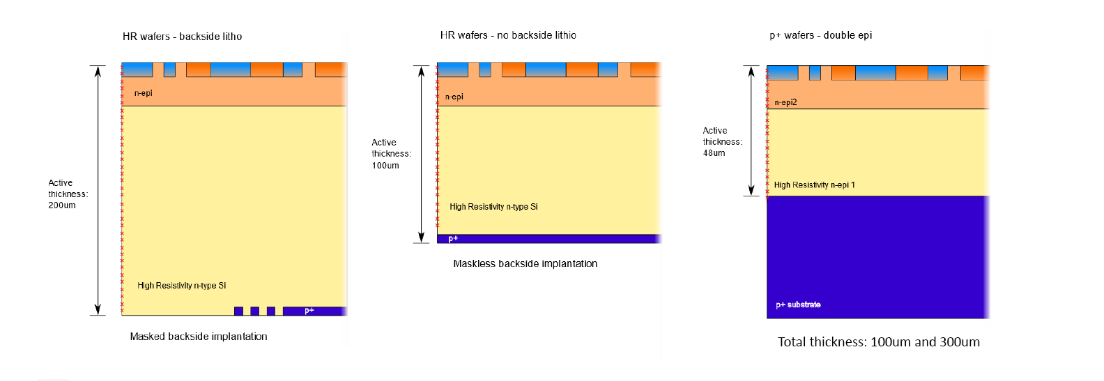
\includegraphics[width=.8\linewidth]{figures/ARCADIA/ARCADIA_substrate.png}
        \caption{}
        \label{fig:ARCADIA_substrate}
    \end{figure}

    Wafer thinning and backside litography were necessary to introduce a junction at the bottom surface, used to bias the substrate to full depletion while maintaining a low voltage at the front side.  \\
    C'è un deep pwell per - priority chain separare l'elettronica dal sensore; per controllare il punchthought
    è stato aggiunto un n doped epitaxial layer having a resistivity lower than the substrate.
    It is part of the cathegory of DMAPS
    Small electrode to enhance the signal to noise ratio.
    It is operated in full depletion with fast charge collection by drift.

    \subsection{Two different FE flavor}

        Le differenze tra Alpide e bulk driven sono un po' più complesse di quanto
        hai scritto.
        Si tratta proprio di due architetture diverse.
        Il primo amplifica il segnale attraverso il trasferimento di carica tra
        due capacità.
        Nel bulk driven invece il guadagno è dato dal rapporto tra due
        transconduttanze. Inoltre ci sono altre differenze, il bulk driven è più sensibile alle cadute di tensione sul ground (che ahimè è esattamente ciò che accade nei dimostratori che abbiamo ora, a causa dell'anomalo consumo di corrente dal digitale, altro baco che abbiamo corretto nella terza sottomissione).
        Anche i livelli di tensione nei nodi interni dei due front-end differiscono e il meccanismo di clipping che funzionava per l'Alpide non è applicabile al bulk driven. Di conseguenza abbiamo un bias in più (ICLIP) nel secondo flavour per controllare il clipping. Nell'Alpide il clipping c'è, ma l'architettura usata permette di non aver bisogno di un bias esterno, anche se in una versione di Alpide di ALICE hanno scelto di controllare comunque la corrente di clip esternamente, per una maggiore flessibilità. Infine alcuni bias che hanno lo stesso nome nei due flavour, perché svolgono la stessa funzione, differiscono nel valore di configurazione didefault.
        

        


\section{Readout logic and data structure}
    In order to achieve the lowest possible power consumption, the matrix is clockless, no free-running clock, and to save as much area as possible, it will not buffer any hits, and its readout will thus be triggerless.

    The Periphery has both an analog part, segmented per Section, and a digital part, which is instead shared. The analog part hosts the bias cells for the AFE dei pixel, mentre la parte digitale che è unica per tutti riprocessa le hit che vengono dalle sezioni e 8b10b encode le parole per data transmittion.  
    %Sections with own 320MHz DDR Output link. The sections will have to have their own output link, in order to ease future up-scaling.-> lo dicono come requirement
    
    
    \subsection{Matrix division and data-packets}
        The matrix is divided into an internal physical and logical hierarchy:
        The 512 columns are divided in 16 section: 512$\times$32 pixels, each section has different voltage-bias + serializzatori.
        Each section is devided 512$\times$2 column, and in 32$\times$2 core: in modo che in ogni doppia colonna ci siano 1Pacchetto dei dati  6 cores. ricordati dei serializzaatori: sono 16 ma possono essere ridotti ad uno in modalità spazio
        Ed infine regioni da 4$\times$2
        \begin{figure}[h!]
            \centering
            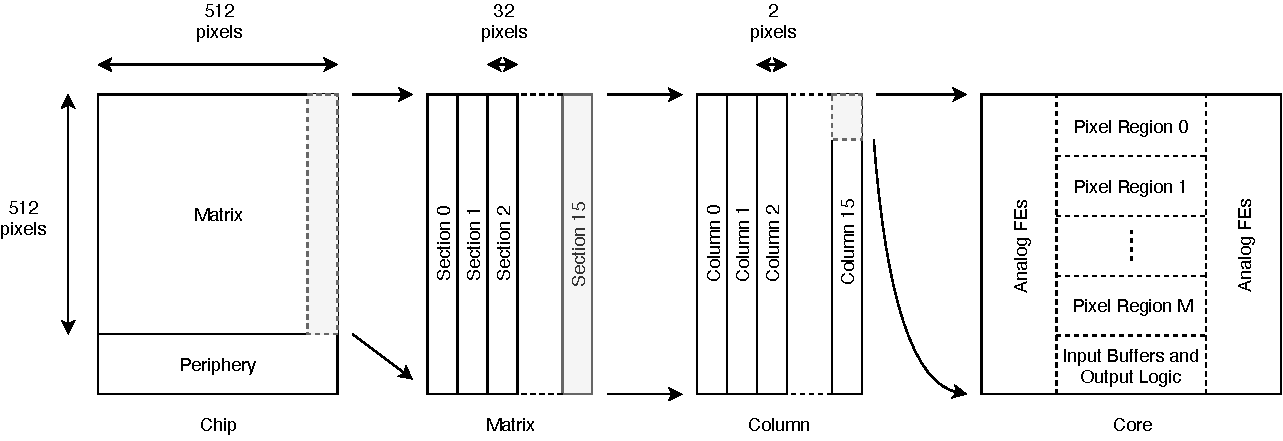
\includegraphics[width=.95\linewidth]{figures/ARCADIA/hierarchy.pdf}
            \caption{}
            \label{fig:hierarchy}
        \end{figure}
        The readout design must be capable of addressing the following matters Enough bus bandwidth for a hit rate of 100 MHz/cm2. Design decisions: Try and send as much data as possible to the periphery (bandwidth)
        Lowest amount of logic possible (more routability)
        
        \begin{figure}[h!]
            \centering
            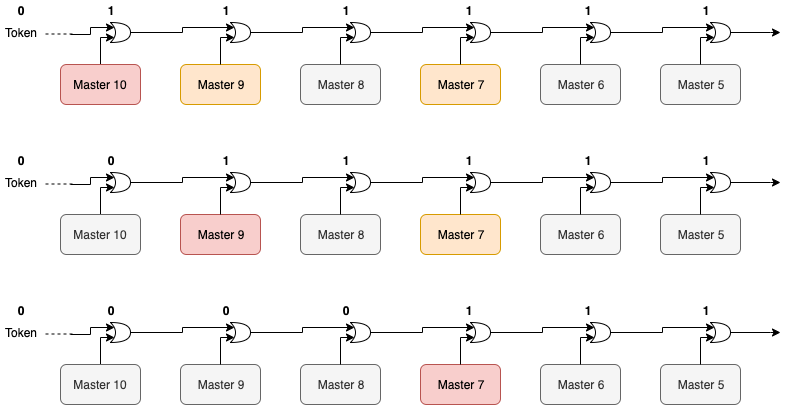
\includegraphics[width=.95\linewidth]{figures/ARCADIA/token_chain.png}
            \caption{}
            \label{fig:token_chain}
        \end{figure}


        \begin{figure}[h!]
            \centering
            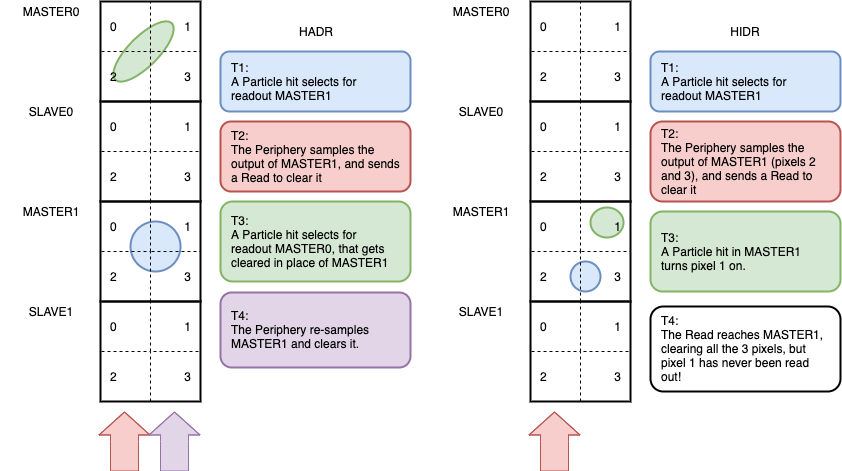
\includegraphics[width=.95\linewidth]{figures/ARCADIA/hadrhidr.png}
            \caption{}
            \label{fig:hadrhidr}
        \end{figure}
        


        \begin{figure}[h!]
            \centering
            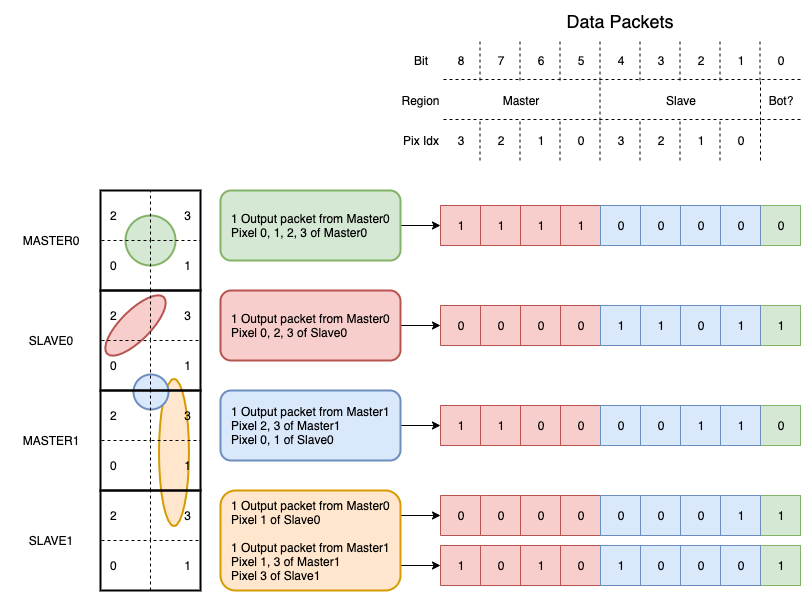
\includegraphics[width=.95\linewidth]{figures/ARCADIA/clustering.png}
            \caption{}
            \label{fig:clustering}
        \end{figure}

        \begin{figure}[h!]
            \centering
            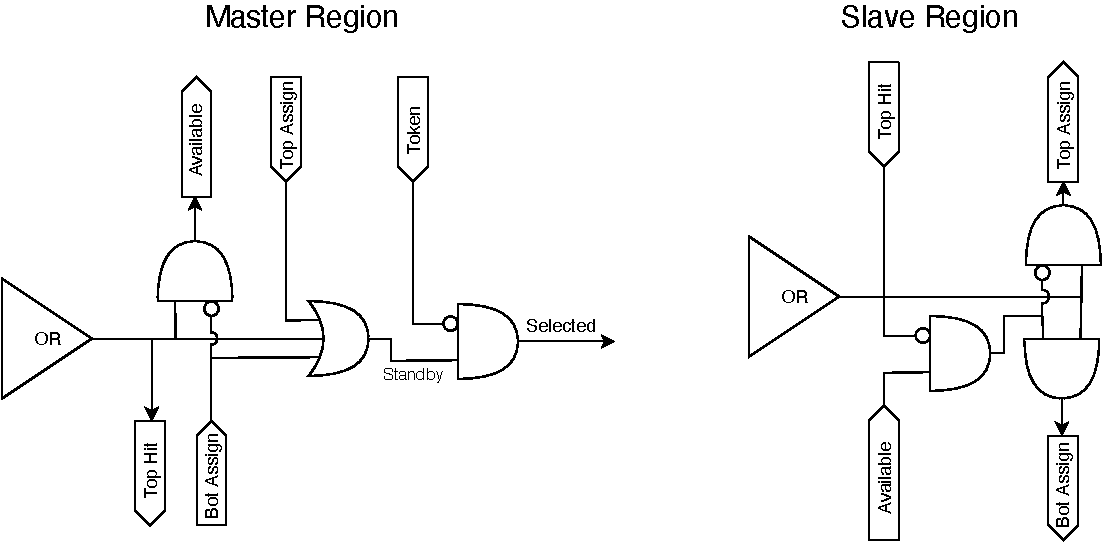
\includegraphics[width=.95\linewidth]{figures/ARCADIA/clustering_logic.pdf}
            \caption{}
            \label{fig:clustering_logic}
        \end{figure}
        


        Questa divisione si rispecchia in come sono fatti i dati: scrivi da quanti bit un
        dato è fatto e le varie cordinate che ci si trovano dentro; devi dire che c'è un pixel hot
        e spieghi dopo a cosa serve, e devi accennare al timestamp

        "A core is simply the smallest stepped and repeated instance of digital circuitry.
        A relatively large core allows one to take full advantage of digital sybthesis tools
        to implement complex functionality in the pixel matrix, sharing resources among
        many pixels as needed.".
        pagina 28 della review.\\



        TABELLA: con la gerarchia del chip
        Matrix (512x512 pixels)
        Section (512x32 pixels)
        Column (512x2)
        Core (32x2)
        Region (4x2)

        Nel chip trovi diverse padframe: cosa c'è nelle padframe e End of section.

        "DC-balance avoids low frequencies by guaranteeing at least one transition every
        n bits; for example 8b10b encoding n =5"

